\begin{figure}[h!]
	\begin{center}
		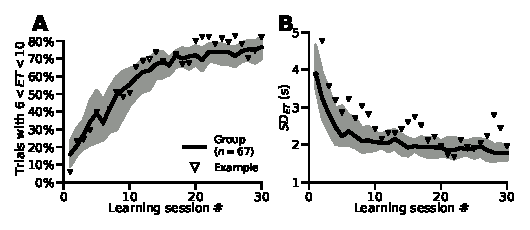
\includegraphics[scale=1]{ch-appendicies/figures/CorrectTrialCurve.pdf}
		\caption[Task Performance Improvement]
		{\textbf{Task performance improvement across sessions.}
		\textbf{A)} Percentage of trials in which animals entered the reward area close to GT ($6~s<ET<10~s$), session-by-session.
		\textbf{B)} Session-by-session standard deviation of ET.
		Triangles show performance improvement for an example animal (same animal as in \autoref{fig:lesion:task}).
		}
		\label{fig:appendix:CorrectTrialCurve}
	\end{center}
\end{figure}